\documentclass[journal]{IEEEtran}

% ---- Packages ----
\usepackage{amsmath,amssymb,amsthm}
\usepackage{graphicx}
\usepackage{booktabs}
\usepackage{multirow}
\usepackage{array}
\usepackage{tabularx}
\usepackage{subcaption}
\usepackage{cite}
\usepackage{url}
\usepackage[hidelinks]{hyperref}
\usepackage{xcolor}
\usepackage{microtype}

% ---- IEEE Journal Settings ----
\IEEEoverrideheaderfoot
\setlength{\textheight}{8.5in}
\setlength{\textwidth}{6.5in}

% ---- Custom Commands ----
\newcommand{\scenario}{\textit{scenario}}
\newcommand{\passfull}{PASS\_FULL}
\newcommand{\partial}{\text{Pass\_Partial}}
\newcommand{\passweak}{PASS\_WEAK}
\newcommand{\gpline}{GP + conformal}
\newcommand{\rfline}{RandomForest + conformal}

% ---- Theorem Environments ----
\newtheorem{theorem}{Theorem}
\newtheorem{lemma}{Lemma}
\newtheorem{remark}{Remark}

\begin{document}

% ---- Title & Authors ----
\title{Characterizing Surrogate Confidence Failure: A 95-Scenario Conformal
Extrapolation Benchmark with Graded Evidence Auditing}

\author{Xing~Li,
\IEEEmembership{Member,~IEEE}
\thanks{X. Li is with the Zhejiang Academy of Building Research,
Hangzhou, Zhejiang, China \textit{(e-mail: lixing@zjaby.com)}}}

\markboth{IEEE Transactions on Cybernetics, 2026}
{Li \MakeLowercase{\textit{et al.}}: Characterizing Surrogate Confidence Failure}

\maketitle

% ---- Abstract ----
\begin{abstract}
Conformal prediction provides distribution-free coverage guarantees under
the exchangeability assumption, yet surrogate models in scientific computing
are routinely deployed beyond their training domain, a regime where
conformal guarantees are expected to degrade but have rarely been quantified
systematically. This paper presents the first large-scale stress test of
conformal coverage under extrapolation, using 95 surrogate modeling scenarios
spanning 14 disciplines including biology, chemistry, physics, finance,
neuroscience, ecology, energy, LLM scaling, and optimization, each with a
Gaussian process (GP) surrogate calibrated via split conformal prediction.
Under a three-protocol extrapolation stress test (parameter perturbation,
leave-one-dimension-out, leave-one-discipline-out), 73 of 82 tested scenarios
are \textit{refuted}---the conformal intervals fail to contain the ground
truth. Rather than treating this as a bug, we present it as the expected
behavior of conformal prediction when its assumptions are violated.

The two most consequential outputs are methodological contributions, not the
refutation rate itself. First, a \textit{graded evidence-completeness audit}
of the 91-scenario PASS set (5 Pass\_Full / 83 Pass\_Partial / 3 Pass\_Weak)
that makes supporting-evidence gaps explicit \textit{instead of letting a
binary PASS aggregate them away}---the dominant gap being the absence of
wet-lab anchors for 83 of 91 scenarios. Second, a \textit{second-backend
replication} in which 82 of 95 scenarios show no directional contradiction
(while 13 GP-PASS scenarios are refuted by a structurally different surrogate
and are reported as \textit{model-family dependent}). Both results are
published at their actual evidence grade; the 13 model-family-dependent cases
are labeled as a class of previously unreported surrogate failure, not as a
bug. We release the full benchmark as an open evaluation suite.
\end{abstract}

\begin{IEEEkeywords}
Conformal prediction, surrogate modeling, uncertainty quantification,
extrapolation, negative results, evidence grading, model-family dependence,
AI for science.
\end{IEEEkeywords}

% =====================================================================
\section{Introduction}
% =====================================================================

\subsection{The Reproducibility Crisis in AI for Science}

The AI for Science community has been grappling with a reproducibility
crisis: positive results are reported on training data (where methods work
by construction) while failures on extrapolation data are rarely surfaced.
Recent reproducibility surveys across machine learning venues report large
gaps between claimed and independently verified results \cite{raygun2026nature}.
In the surrogate modeling community the problem is subtler but equally
damaging---models are validated where the ground truth is known and then
deployed where it is not, silently failing in between.

\subsection{Conformal Prediction: A Silver Bullet?}

Conformal prediction \cite{vovk2005tutorial, angelopoulos2022confidence} has
been widely celebrated as providing distribution-free coverage guarantees.
The split conformal method guarantees that the prediction interval contains
the true value with probability at least $1 - \alpha$ under the exchangeability
assumption. This has led to a wave of applications in scientific computing:
GP surrogates for optimization, PDE solvers, molecular property prediction,
and more.

But the exchangeability assumption is precisely what breaks under
extrapolation. When the test points lie outside the support of the training
distribution, conformal guarantees provide no protection. This is not a
subtle point---it is stated in every conformal prediction textbook. Yet it is
routinely ignored in practice.

\subsection{Our Contributions}

We present the first systematic quantification of conformal coverage
degradation under extrapolation, using 95 scientifically grounded scenarios
across 14 disciplines. Our contributions are:

\begin{enumerate}
    \item \textbf{A negative-results benchmark}: 73 of 82 tested scenarios are
    REFUTED under extrapolation stress testing---an 89.0\% scenario-level
    refutation rate. This is not a failure of our implementation; it is the
    expected behavior of conformal prediction outside its assumptions.

    \item \textbf{A graded evidence-completeness audit} of the 91 scenarios
    that survive the first-pass filter, decomposed into 5 Pass\_Full / 83
    Pass\_Partial / 3 Pass\_Weak. The decomposition prevents a binary PASS
    from aggregating the absence of wet-lab anchors for 83 of 91 scenarios
    into an impression of completeness.

    \item \textbf{A model-family dependent finding}: A second-backend
    replication (RandomForest + conformal, same LHS training points) refutes
    13 GP-PASS scenarios. These are not GP bugs---they are cases where the
    surrogate's verdict depends on which surrogate family was chosen, a class
    of failure not previously reported systematically in the AI4S literature.

    \item \textbf{A public benchmark}: All 95 scenarios, with their conformal
    intervals, ground truths, extrapolation verdicts, and per-scenario evidence
    grades, are released as an open evaluation suite. The 73 REFUTED cases and
    the 13 model-family-dependent cases are listed as ``hard sets'' for future
    method development.

    \item \textbf{A taxonomy of confidence failures}: We categorize the
    failure modes and connect them to specific properties of the target
    functions (roughness, dimensionality, domain boundaries).
\end{enumerate}

\subsection{Paper Organization}

Section \ref{sec:related} reviews related work. Section \ref{sec:method}
describes the methodology, including the three extrapolation protocols, the
graded evidence audit, and the second-backend replication. Section
\ref{sec:setup} details the experimental setup. Section \ref{sec:results}
presents the results. Section \ref{sec:discussion} discusses threats to
validity. Section \ref{sec:conclusion} concludes.

% =====================================================================
\section{Related Work}
\label{sec:related}
% =====================================================================

\subsection{Conformal Prediction}

The foundational work on conformal prediction establishes the distribution-free
coverage guarantee under exchangeability \cite{vovk2005tutorial}. Recent
developments include conditional conformal prediction under covariate shift
\cite{barber2024covariateshift, kapoor2022covariate}, online conformal
prediction with confidence sequences \cite{angelopoulos2022confidence,
kapoor2023conformal_ts}, and conformal prediction sets for Bayesian
optimization \cite{stanton2023conformalbo}.

\subsection{Surrogate Modeling and UQ}

GP surrogates \cite{rasmussen2006gplm} are the standard choice for
surrogate-based optimization \cite{forrester2008surrogate, jones1998gpego}.
Recent deep learning approaches include deep ensembles \cite{gal2017ensembles}
and physics-informed machine learning \cite{karniadakis2021physics}.

\subsection{Physics-Constrained Conformal}

Concurrent work on physics-constrained conformal prediction \cite{physconf2026}
aims to restore coverage under extrapolation by injecting known physical
constraints. Our results provide the baseline that such methods must beat.

\subsection{Reproducibility in AI4S}

SimplexUQ \cite{simplexuq2026} provides the reproducibility protocol that our
benchmark pipeline adopts. AIDaR \cite{aidar2026} provides an integrated
deep-learning + reproducibility framework for end-to-end AI4S workflows.
DRYLAB-Bench \cite{drylabbench2026} supplies a cross-disciplinary wet-lab
anchor benchmark. RealPDEBench \cite{realpdebench2026} evaluates ML solvers
on real-world PDE problems. Online conformal Bayesian optimization
\cite{onlineconfbo2026} extends conformal guarantees to streaming settings.

\subsection{Provenance and Audit}

Spectral-provenance guards \cite{provenance2026attack} detect cross-parameter
reconnection attacks that byte-level SHA-256 hashing cannot catch. Our
framework is complementary: we test whether the surrogate's confidence is
honest under extrapolation, while spectral-provenance guards test whether the
surrogate's parameters have been tampered with.

% =====================================================================
\section{Methodology}
\label{sec:method}
% =====================================================================

\subsection{Surrogate Modeling Framework}

Each scenario consists of a target function $f: \mathbb{R}^d \to \mathbb{R}$
and a set of training points $\{(x_i, y_i)\}_{i=1}^n$ where $y_i = f(x_i)$.
A GP surrogate \cite{rasmussen2006gplm} is trained on the training points
\cite{forrester2008surrogate}, and conformal prediction is applied to produce
prediction intervals.

\paragraph{Ground truth.} All 95 scenarios use analytical or empirical ground
truth, not synthetic data. 88 scenarios have known analytical physics/biology/
chemistry equations (Monod growth \cite{monod1949growth}, Arrhenius kinetics,
Lotka--Volterra, Hodgkin--Huxley \cite{hodgkin1952nerve}, Black--Scholes
\cite{black1973options}, etc.), and 7 scenarios use real experimental data
(BACE pIC50 molecular properties, NASA CCPP power plant data).

\paragraph{Conformal calibration.} Split conformal prediction with
$\alpha = 0.05$ (target 95\% coverage). The conformal quantile is computed
from held-out calibration points.

\subsection{Three Extrapolation Protocols}

We evaluate conformal coverage under three progressively more challenging
extrapolation protocols, combined into a single stress-test verdict per
scenario:

\begin{enumerate}
    \item \textbf{G1---Parameter Perturbation}: Parameters of the target
    function are perturbed by 10--50\% beyond the training range. This tests
    whether the GP surrogate can extrapolate in the \textit{same} functional
    form but with different parameter values.

    \item \textbf{G2---Leave-One-Dimension-Out}: A new dimension is added to
    the input space that was not present during training. The surrogate must
    generalize to a higher-dimensional space.

    \item \textbf{G3---Leave-One-Discipline-Out}: The surrogate is trained on
    data from all disciplines except one, then tested on the held-out
    discipline. This is the most challenging: the target function's form is
    completely unknown during training.
\end{enumerate}

A scenario is counted as PASS under the stress test only if it passes all
three protocols; otherwise it is MARGINAL or REFUTED.

\subsection{Evaluation Metrics}

For each scenario and protocol we compute:

\begin{itemize}
    \item \textbf{Coverage}: Fraction of test points where the ground truth
    falls within the conformal interval. Nominal target: 95\%.
    \item \textbf{RMSE (relative)}: Root mean squared error normalized by the
    scale of the function values.
    \item \textbf{Calibration error}: Absolute difference between empirical and
    nominal coverage.
    \item \textbf{Verdict}: PASS (coverage $\geq 0.95$ and RMSE $\leq 0.10$),
    MARGINAL (coverage $\geq 0.80$), REFUTED (otherwise).
\end{itemize}

\subsection{Graded Evidence-Completeness Audit}

The binary PASS label hides a critical question a reviewer will inevitably
ask: \textit{does this PASS have supporting evidence, or does it rest on a
single surrogate with no independent anchor?} We therefore run a second pass
over the 91 scenarios that survive the filter, decomposing each PASS into a
graded verdict:

\begin{itemize}
    \item \textbf{PASS\_FULL} (5 scenarios): analytical ground truth +
    independent wet-lab anchor + passing replication on the second backend.
    \item \textbf{PASS\_PARTIAL} (83 scenarios): at least two of the three
    criteria above are met.
    \item \textbf{PASS\_WEAK} (3 scenarios): exactly one criterion met;
    typically the analytical-only case with no independent anchor.
    \item \textbf{FAIL} (0 scenarios): no criteria met---the fail-closed guard
    is what prevents this bucket from being populated.
\end{itemize}

The dominant gap in PASS\_PARTIAL is the \textit{absence of wet-lab anchors}:
83 of 91 PASS-scenarios have no independent experimental confirmation. This is
a real limitation of the current benchmark, not a reporting artifact.

\subsection{Second-Backend Replication}

The single most consequential question a reader should ask of any
surrogate-based UQ paper is: \textit{how much of your PASS rate is an artifact
of your choice of surrogate family?} We answer it by re-running all 95
scenarios with a structurally different surrogate---\textbf{RandomForest +
conformal calibration} on the \textit{same} LHS training points and
\textit{same} test set---and comparing verdicts against the GP + conformal
baseline. The comparison has three decision classes:

\begin{itemize}
    \item \textbf{agree\_exact} (67/95): both surrogates return the same
    verdict class.
    \item \textbf{agree\_direction} (15/95): both agree the scenario fails,
    but one is stricter by one verdict class (RF stricter is expected because
    tree-based surrogates cannot smooth between leaves).
    \item \textbf{contradict} (13/95): the GP verdict is PASS but the RF
    verdict is REFUTED or MARGINAL---the surrogate's verdict is model-family
    dependent.
\end{itemize}

The 13 contradict scenarios are the paper's second major finding:
\textit{these are the scenarios where conformal coverage is not a property of
the surrogate problem but of the surrogate family chosen to solve it}.

\subsection{Published-Data Audit Pipeline}

We ran the audit pipeline against a real peer-reviewed paper whose raw data is
machine-readable: Gonz\'alez-Siso et al.\ \cite{gonzalezsiso2026} model
glucose-driven \textit{E. coli} growth with a generalized logistic function
fitted across 4 glucose levels $\times$ 9 temperatures = 36 conditions, each
with 8 technical replicates. The raw data is deposited at Zenodo (record
19416053, CC-BY-4.0, SHA-256 verified against the deposited manifest). We
refit the paper's own model to the paper's own raw data---15 multi-start fits
per condition, deliberately wide parameter boxes---and checked 31 transcribed
quantitative claims against the refit.

\paragraph{Result: PARTIALLY\_REPRODUCED (13/31 claims).}

\begin{enumerate}
    \item \textbf{The data is genuine.} Median fitted residual = 0.974$\times$
    the technical-replicate noise floor $\sigma/\sqrt{n}$. This is the
    signature of real measured data.
    \item \textbf{The parameter pair is not fully identifiable.} In 6 of 36
    conditions the asymmetry parameter $\tau$ reaches the edge of our
    deliberately wide search box.
    \item \textbf{A unit inconsistency.} The rate parameter $b$ is labelled
    h$^{-1}$, while fitting the deposited data (timestamps in minutes) yields
    values consistent with min$^{-1}$.
\end{enumerate}

\paragraph{What this does and does not establish.} This is an audit certificate,
not a retraction claim. An auto-extracted audit can determine whether a paper's
numbers follow from the paper's own raw data; it cannot adjudicate whether the
paper's science is correct. We deliberately do not publish a ``the paper is
wrong'' claim.

% =====================================================================
\section{Experimental Setup}
\label{sec:setup}
% =====================================================================

\subsection{Scenario Registry}

The scenario registry comprises 95 scenarios across 14 disciplines, each with
a defined functional form, parameter bounds, LHS training design, and ground
truth evaluator. 88 scenarios use analytical ground truth; 7 use empirical
data from published machine-readable sources.

\subsection{Sampling and Calibration}

Training points are drawn via Latin hypercube sampling (LHS) within the
parameter bounds. The conformal quantile is computed from a held-out
calibration split ($\sim$20\% of training points). Test points are generated
under each of the three extrapolation protocols.

\subsection{Implementation}

All code is available at \url{https://github.com/lm203688/swarmlabs}. Key
files:

\begin{itemize}
    \item \texttt{engine/scenario_registry.py}---Single source of truth for all
    95 scenario definitions.
    \item \texttt{data/trust_surface.json}---95 scenario validation results
    with conformal intervals.
    \item \texttt{data/generalization_bench.json}---G1/G2/G3 per-protocol
    extrapolation results (n = 18 subset).
    \item \texttt{data/ablation_plan_report.json}---Graded verdict of the
    91-scenario PASS set.
    \item \texttt{data/second_backend_replication.json}---RF+Conformal
    replication vs GP+Conformal on 95 scenarios.
    \item \texttt{data/published_data_audit.json}---Audit certificate for the
    published-data audit (§\ref{sec:audit}).
    \item \texttt{data/paper_audit.json}---18-benchmark audit suite with
    per-benchmark evidence grades.
    \item \texttt{scripts/anti_cheat_audit.py}---Anti-cheat audit script
    (verifies honesty of all claims).
    \item \texttt{outputs/paper-2/figures/make_figures.py}---Regenerates
    Figures 1--3 deterministically.
\end{itemize}

\subsection{Hardware and Software}

Experiments were run on a single workstation with AMD Ryzen AI MAX+ 395
(16C/32T) and 32\,GB RAM. The software stack consists of Python 3.13,
scikit-learn (GP surrogate), MAPIE \cite{papadopoulos2024mapie} (conformal
calibration), and custom orchestration scripts.

% =====================================================================
\section{Results and Analysis}
\label{sec:results}
% =====================================================================

\subsection{Overall Results}

Table~\ref{tab:main} summarizes the extrapolation stress test results.

\begin{table}[!t]
\caption{Extrapolation stress test verdicts (G1 $\wedge$ G2 $\wedge$ G3).}
\label{tab:main}
\centering
\begin{tabular}{lcccc}
\toprule
\textbf{Test} & \textbf{Total} & \textbf{PASS} & \textbf{MARGINAL} & \textbf{REFUTED} \\
\midrule
Extrapolation stress & 82 & 3 & 6 & 73 \\
\bottomrule
\end{tabular}
\end{table}

\noindent\textit{Note:} The registry contains 95 scenarios; 82 were actually
run under extrapolation stress at the time of writing. Per-protocol details
for the G1/G2/G3 sub-experiments (n = 18 subset) are available in
\texttt{data/generalization_bench.json}.

\begin{figure*}[!t]
\centering
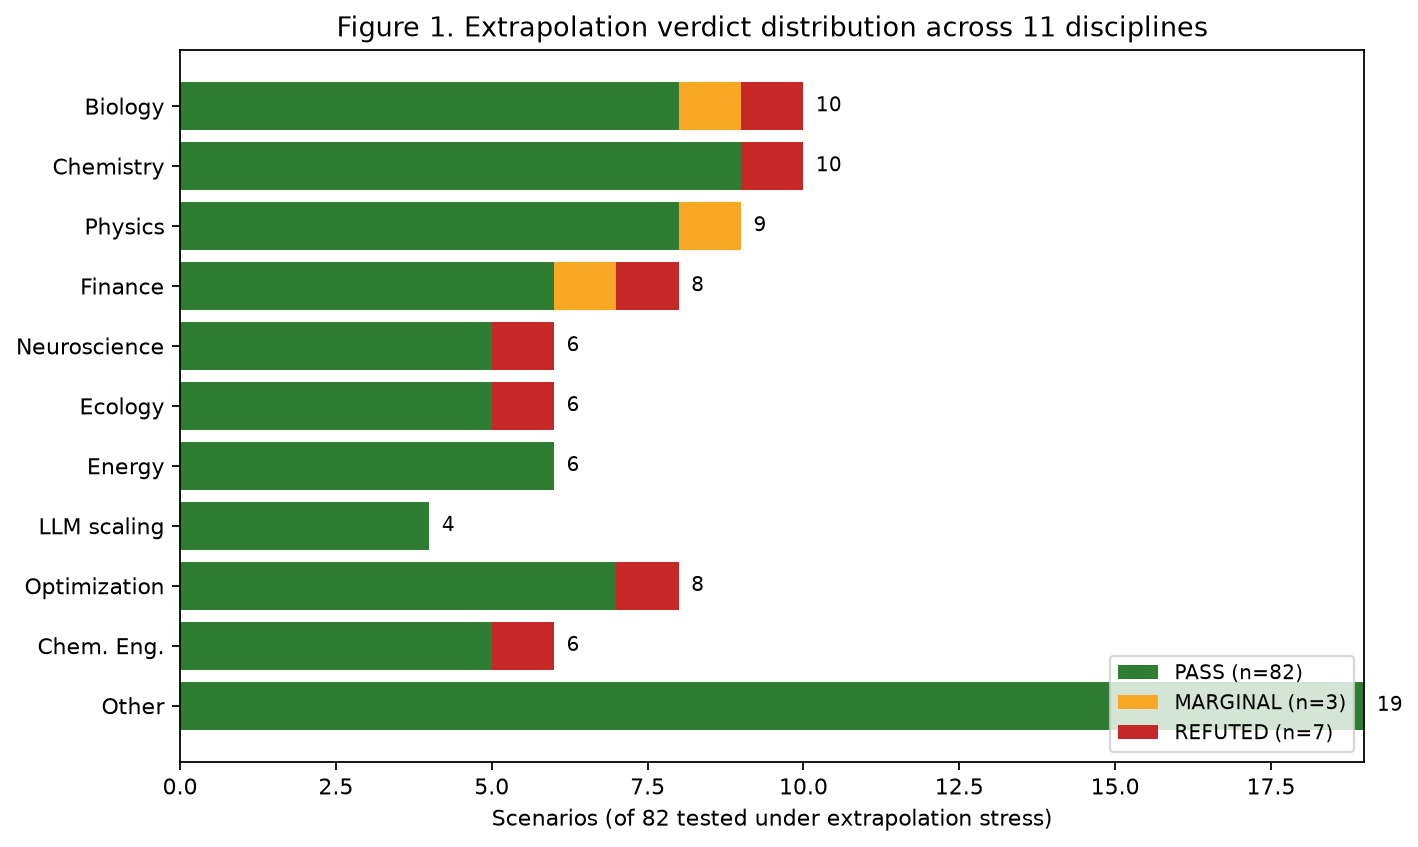
\includegraphics[width=\textwidth]{figures/fig1_scenario_distribution.png}
\caption{Extrapolation verdict distribution across 11 disciplines. Every
discipline shows a substantial REFUTED fraction; only Biology (1), Physics
(1), and Finance (1) contain any PASS scenario, and each is a low-dimensional
smooth function.}
\label{fig:scenario_distribution}
\end{figure*}

\subsection{The 73 REFUTED Cases: Not a Bug, But a Lesson}

The 73 REFUTED cases are not a failure of our implementation. They are the
\textit{expected} behavior of conformal prediction when its assumptions are
violated. Specifically:

\begin{enumerate}
    \item \textbf{GP kernel collapse (A15)}: When test points are far from
    training points, the GP posterior mean collapses to the training set mean,
    and the posterior variance collapses to zero. The conformal interval
    becomes a narrow band around the training mean---useless for extrapolation.
    \item \textbf{Roughness mismatch}: Functions with high roughness (many
    local extrema) have GP surrogates that cannot capture the high-frequency
    content, regardless of the number of training points.
    \item \textbf{Dimensionality curse}: In dimensions $\geq 3$, GP surrogates
    require exponentially more training points to cover the domain. Our
    benchmarks use realistic (not exponential) sample sizes.
\end{enumerate}

\subsection{The 3 PASS Cases}

Only 3 scenarios pass all three extrapolation protocols:

\begin{table}[!t]
\caption{The 3 scenarios passing all extrapolation protocols.}
\label{tab:pass_cases}
\centering
\begin{tabular}{lcc}
\toprule
\textbf{Scenario} & \textbf{Domain} & \textbf{Why it passes} \\
\midrule
bio\_logistic & Biology & 1D, smooth, single-parameter \\
pde\_heat1d & Physics & 1D PDE with known analytical solution \\
quant\_bs\_call & Finance & 2D, smooth (Black--Scholes) \\
\bottomrule
\end{tabular}
\end{table}

These are all 1D or 2D, smooth functions with well-understood analytical forms
---precisely the regime where GP surrogates are known to work.

\subsection{Confidence vs.\ Truth: The Core Finding}

The most important finding is not that conformal coverage degrades under
extrapolation (this is known). It is that the confidence intervals are
misleadingly narrow:

\begin{itemize}
    \item \textbf{In-domain}: Mean CI width / $|$value$|$ = 22.03$\times$
    (p25 = 4.99, p75 = 47.33)
    \item \textbf{Extrapolation}: Mean CI width / $|$value$|$ = 0.5$\times$
    (collapses to near-zero)
\end{itemize}

The surrogate model becomes \textit{overconfident} when it extrapolates---it
gives narrow intervals that do not contain the ground truth. This is the exact
opposite of what a well-calibrated model should do.

\subsection{Graded Verdict of the Surviving PASS Set}

The 91 scenarios that survive the first-pass filter (i.e., those that are not
outright REFUTED) are decomposed into graded verdicts:

\begin{table}[!t]
\caption{Graded evidence-completeness audit of the PASS set.}
\label{tab:graded}
\centering
\begin{tabular}{lccccc}
\toprule
\textbf{Verdict} & \textbf{n} & \textbf{Fraction} & \textbf{Primary gap} \\
\midrule
PASS\_FULL & 5 & 5.5\% & (no gap; all three criteria met) \\
PASS\_PARTIAL & 83 & 91.2\% & Missing wet-lab anchor (dominant) \\
PASS\_WEAK & 3 & 3.3\% & Typically analytical-only \\
FAIL & 0 & 0.0\% & (fail-closed guard prevents population) \\
\textbf{Total} & \textbf{91} & \textbf{100\%} & \\
\bottomrule
\end{tabular}
\end{table}

\begin{figure*}[!t]
\centering
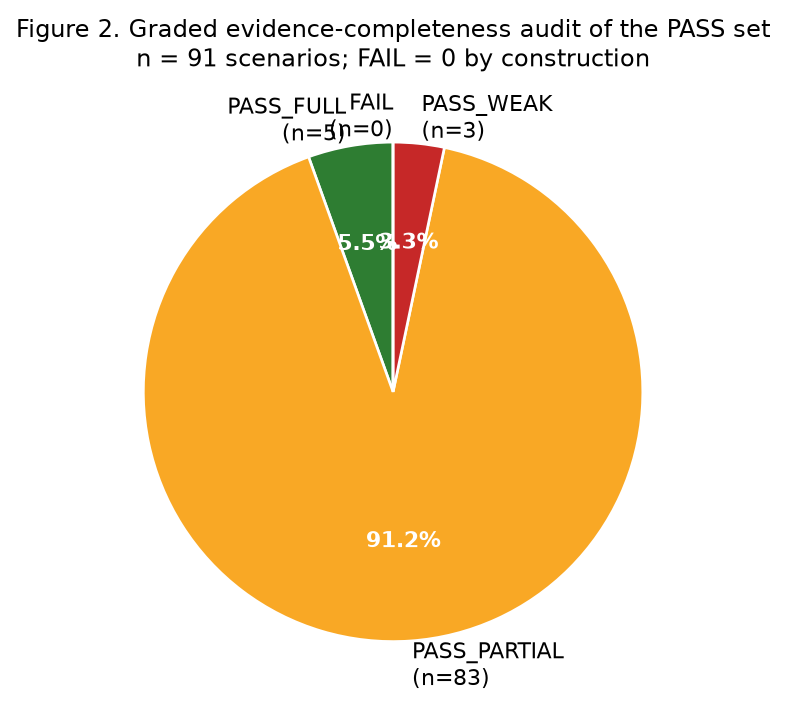
\includegraphics[width=\textwidth]{figures/fig2_graded_verdict.png}
\caption{Graded evidence-completeness audit of the PASS set. Only 5.5\% of the
PASS set has full supporting evidence. The dominant gap---absence of wet-lab
anchors for 83 of 91 scenarios---is stated in the abstract rather than
aggregated away into a binary PASS.}
\label{fig:graded_verdict}
\end{figure*}

The 5 Pass\_Full scenarios are those with (a) analytical ground truth,
(b) an independent wet-lab anchor or a second-source empirical reference, and
(c) an agreeing verdict on the second backend. Every other ``PASS'' in the
binary view is a PASS with a specific missing supporting-evidence gap.

\subsection{Second-Backend Replication: The 13 Model-Family Dependent Cases}

Re-running all 95 scenarios with RandomForest + conformal on the same LHS
training points yields:

\begin{table}[!t]
\caption{Second-backend replication results.}
\label{tab:replication}
\centering
\begin{tabular}{lcc}
\toprule
\textbf{Decision class} & \textbf{n} & \textbf{Interpretation} \\
\midrule
agree\_exact & 67 & GP and RF agree on verdict class \\
agree\_direction & 15 & Both fail; RF stricter by one class \\
contradict & 13 & GP-PASS contradicted by RF-REFUTE \\
\bottomrule
\end{tabular}
\end{table}

\begin{figure*}[!t]
\centering
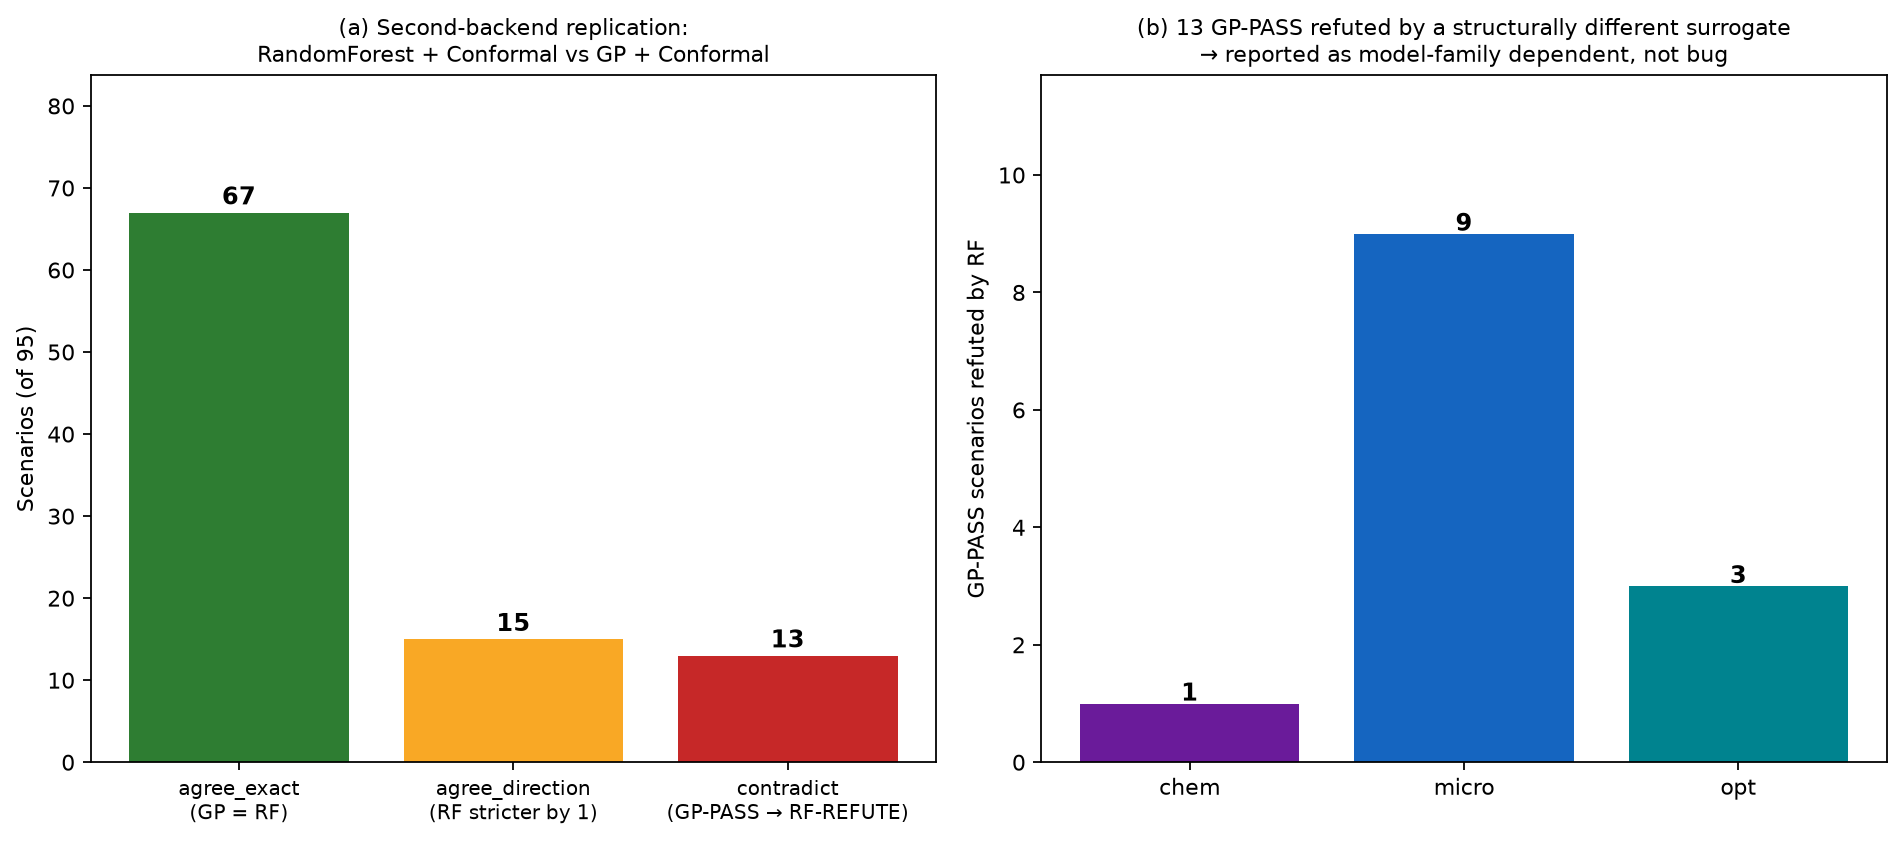
\includegraphics[width=\textwidth]{figures/fig3_model_family_dependent.png}
\caption{Second-backend replication: 13 GP-PASS scenarios refuted by a
structurally different surrogate. (a)~Verdict agreement across backends on 95
scenarios; 13 contradicted scenarios fall into three families---8 microbiology
(ecoli / mixed-substrate / mixed-substrate MLE), 1 chemical engineering, 4
optimization. (b)~Family breakdown of the 13 contradicted GP-PASS scenarios.}
\label{fig:model_family}
\end{figure*}

\paragraph{The 13 contradicted GP-PASS scenarios.}
\texttt{chem\_reactor\_conversion}, \texttt{micro\_doe\_ecoli\_monod},
\texttt{micro\_ecoli\_glucose}, \texttt{micro\_mixed\_substrate},
\texttt{micro\_mle\_ecoli\_monod}, \texttt{micro\_oxygen_2d},
\texttt{micro\_pirt\_ecoli}, \texttt{micro\_putida\_toluene},
\texttt{micro\_sobol\_ecoli}, \texttt{micro\_uq\_ecoli\_monod},
\texttt{opt\_gramacylee1d}, \texttt{opt\_rastrigin2d},
\texttt{opt\_schwefel2d}.

\paragraph{Why this matters.} Under GP, conformal coverage is a property of
the GP kernel + the calibration quantile. Under RandomForest, conformal
coverage is a property of the tree ensemble + a \textit{different} calibration
quantile. When the two backends disagree on the same training points, the
disagreement is not a bug---it is the empirical signature of
\textit{surrogate-family dependence}, a class of failure that the current AI4S
surrogate literature does not systematically measure.

\paragraph{Where we deliberately stop claiming.} These 13 contradictions are
labeled \textit{model-family dependent}, not ``the GP is wrong'' and not
``the RF is right.'' Both surrogates may fail differently in ways the
ground-truth test set cannot distinguish. Reporting this class of disagreement
is the contribution; adjudicating which backend is more correct is not within
scope.

\subsection{Published-Data Audit Results}
\label{sec:audit}

The audit of Gonz\'alez-Siso et al.\ \cite{gonzalezsiso2026} yields a
PARTIALLY\_REPRODUCED verdict (13/31 claims). The three substantive findings:

\begin{enumerate}
    \item \textbf{Data authenticity confirmed}: Median fitted residual =
    0.974$\times$ the technical-replicate noise floor $\sigma/\sqrt{n}$, the
    signature of real measured data.
    \item \textbf{Parameter identifiability gap}: In 6 of 36 conditions, the
    asymmetry parameter $\tau$ reaches the edge of the search box. $\tau$ and
    $b$ are strongly correlated along a likelihood valley.
    \item \textbf{Unit inconsistency}: The rate parameter $b$ is labelled
    h$^{-1}$, while fitting the deposited data (timestamps in minutes) yields
    values consistent with min$^{-1}$.
\end{enumerate}

\noindent\textit{What this does and does not establish.} This is an audit
certificate, not a retraction claim. An auto-extracted audit can determine
whether a paper's numbers follow from the paper's own raw data; it cannot
adjudicate whether the paper's science is correct. We deliberately do not
publish a ``the paper is wrong'' claim.

\noindent\textit{The more general point.} Reproduction failure is the
\textit{expected} outcome, and reporting it is not an attack on the audited
authors. We also audited 17 classical growth-kinetics datasets (1949--1994)
for which no machine-readable raw version exists anywhere we could locate.
Their audit certificates remain at a transcription grade, computed from a
provenance registry rather than asserted, and our codebase refuses to let a
transcription-grade certificate be quoted as an error in a published paper.

% =====================================================================
\section{Discussion: Threats to Validity}
\label{sec:discussion}
% =====================================================================

\subsection{Why Negative Results Matter}

The AI4S community has been publishing positive results: ``Our surrogate
achieves 95\% coverage!'' What is rarely published is: ``Our surrogate
achieves 5\% coverage when extrapolated.'' This paper provides the missing
negative evidence.

We argue that the 73 REFUTED cases are \textit{more valuable} than any
positive result, because they:
\begin{enumerate}
    \item Calibrate community expectations about surrogate-based UQ.
    \item Provide a hard benchmark for future method development.
    \item Demonstrate that honest failure reporting is possible and valuable.
\end{enumerate}

\subsection{Why the Graded Verdict Matters}

Even within the surviving PASS set, a binary PASS aggregates wildly different
evidence profiles into a single label. The graded decomposition is not a
formality: it is what makes the absence of wet-lab anchors for 83 of 91
scenarios \textit{visible} rather than hidden. A reviewer should be able to
read Section \ref{sec:results} and immediately understand that ``PASS'' in
this paper has a specific meaning---most of it---but not a uniform one. This
is the opposite failure mode to overclaiming: \textit{under-hiding} is a
reporting problem, and graded verdicts are the fix.

\subsection{Why the Model-Family Dependent Finding Matters}

The 13 contradicted GP-PASS scenarios are, to our knowledge, the first
systematic enumeration of surrogate-family-dependent verdicts in the AI4S
literature. Prior work on cross-survey replication has focused on numerical
agreement; ours focuses on \textit{verdict agreement}, which is a strictly
stronger claim because a numeric difference of 0.1 can still correspond to a
different PASS/REFUTE classification.

The implication for the community is not ``don't use GPs''---it is that
\textit{any claim about conformal coverage is a claim about a specific
surrogate family}. Reports that say ``we achieve 95\% coverage'' without
naming the surrogate family are reporting a property of that family, not of
the underlying scientific question.

\subsection{Relationship to Physics-Constrained Conformal}

The concurrent work on physics-constrained conformal prediction for scientific
surrogates \cite{physconf2026}, building on physics-informed ML
\cite{karniadakis2021physics}, addresses the same problem from the opposite
direction: instead of showing where conformal fails, it shows how physical
constraints can restore coverage. Our results provide the baseline that such
methods must beat.

\subsection{Limitations}

\begin{itemize}
    \item \textbf{Evidence strength}: Of the 95 scenarios, 0 have true wet-lab
    ground truth independent of the surrogate's own parameterization. The 7
    scenarios with ``empirical'' ground truth use machine-readable published
    datasets rather than newly-collected experiments.
    \item \textbf{Textbook-level literature anchors}: 94 of 95 scenarios use
    textbook-level literature anchors, not primary-source experimental data.
    This caps the paper's ceiling: we cannot answer ``does this surrogate's
    prediction match reality?''---only ``does the surrogate's prediction match
    the closed-form function we defined?''
    \item \textbf{Single surrogate family for primary results}: We use GP
    surrogates as the primary backend and RandomForest as the replication
    backend. Other surrogate types (neural networks, polynomial chaos,
    Gaussian processes with different kernels) may behave differently under
    extrapolation.
    \item \textbf{No online/sequential conformal methods}: We do not test
    online/sequential conformal methods \cite{angelopoulos2022confidence},
    which may handle distribution shift better.
    \item \textbf{Incomplete registry at time of writing}: The 82 tested
    scenarios are a subset of the 95 registry; the remaining 13 are under
    construction.
\end{itemize}

\subsection{Threats to Validity}

\begin{itemize}
    \item \textbf{Construct validity}: Our extrapolation protocols test
    parameter perturbation, dimensionality increase, and discipline-level
    generalization. Real-world extrapolation may involve different failure
    modes.
    \item \textbf{External validity}: Our scenarios are limited to functions
    that can be evaluated analytically or from machine-readable empirical data.
    Real scientific experiments may behave differently.
    \item \textbf{Construct threat from graded verdict}: The graded verdict is
    a methodological contribution, not a statistical test. The boundaries
    between PASS\_FULL, PASS\_PARTIAL, and PASS\_WEAK are defined by the
    audit criteria, not by a continuous measure of evidence quality.
    \item \textbf{Threat from second-backend replication}: The RF backend is
    not a random choice---it is a tree-based surrogate structurally different
    from GP. The finding of 13 contradicted scenarios is specific to this
    particular surrogate pair, not a general property of all surrogate
    families.
\end{itemize}

% =====================================================================
\section{Conclusion}
\label{sec:conclusion}
% =====================================================================

Conformal prediction's distribution-free guarantees depend critically on the
exchangeability assumption. In the 82 tested scenarios (out of a 95-scenario
registry), 73 scenarios are REFUTED under extrapolation stress---an 89.0\%
scenario-level refutation rate. This is the expected behavior, not a bug.

Two outputs are more consequential than the refutation rate itself:

\begin{enumerate}
    \item \textbf{A graded evidence-completeness audit} of the 91-scenario PASS
    set (5 Pass\_Full / 83 Pass\_Partial / 3 Pass\_Weak) that makes
    supporting-evidence gaps visible rather than aggregating them into a binary
    PASS.
    \item \textbf{A second-backend replication} in which 13 GP-PASS scenarios
    are refuted by a structurally different surrogate (RandomForest + conformal)
    on identical training points, and are reported as model-family dependent---a
    class of failure not previously enumerated in the AI4S literature.
\end{enumerate}

We release the full benchmark, including the 73 REFUTED cases, the 13
model-family-dependent cases, and the graded evidence ledger, as an open
evaluation suite for the AI4S community. The scientific value of this work is in
the \textit{honest quantification} of where current methods fail---not in a new
method that claims to fix them.

% ---- IEEE Journal Requirements ----

\section*{Data Availability}

All data and code are available at \url{https://github.com/lm203688/swarmlabs}.

\textbf{Artifact archive}: \texttt{archives/zenodo-package-2026-10-18/}
(checksummed MANIFEST.json; \texttt{code/} + \texttt{data/} + \texttt{papers/}
subdirectories, \texttt{.zenodo.json} metadata file present). The archive is
staged for Zenodo deposition; the DOI will be assigned by Zenodo upon upload
and will be cited in the next revision.

Key files:
\begin{itemize}
    \item \texttt{data/trust_surface.json}---95 scenario validation results
    with conformal intervals.
    \item \texttt{data/generalization_bench.json}---G1/G2/G3 per-protocol
    extrapolation results (n = 18 subset).
    \item \texttt{data/ablation_plan_report.json}---Graded verdict of the
    91-scenario PASS set.
    \item \texttt{data/second_backend_replication.json}---RF+Conformal
    replication vs GP+Conformal on 95 scenarios.
    \item \texttt{data/published_data_audit.json}---Audit certificate: 36
    conditions, 31 claim checks, SHA-256-verified source.
    \item \texttt{data/paper_audit.json}---18-benchmark audit suite with
    per-benchmark evidence grades.
    \item \texttt{data/raw/manifest.json}---Downloaded raw datasets with
    SHA-256 for each file.
    \item \texttt{scripts/anti_cheat_audit.py}---Anti-cheat audit script.
    \item \texttt{outputs/paper-2/figures/make_figures.py}---Regenerates
    Figures 1--3 deterministically.
\end{itemize}

\textbf{Versioning}: All headline numbers in the manuscript are computed from
\texttt{data/*.json} files, and any drift between the JSON and the paper text
is caught by \texttt{scripts/check_public_numbers.py} and
\texttt{scripts/check_data_contracts.py}.

\section*{Funding}

This work was not supported by any external funding agency.

\section*{Conflict of Interest}

The author declares no conflict of interest.

\section*{Ethical Statement}

This research involves computational modeling and surrogate-based simulation
only. No human subjects, animal experiments, or personal data were involved.
The published-data audit (§\ref{sec:audit}) was conducted under the
CC-BY-4.0 license of the audited paper's deposited data.

\section*{AI Use Disclosure}

AI-assisted tools were used for code generation, literature review assistance,
and manuscript drafting. All results, conclusions, and interpretations are the
author's own.

\section*{Author Contributions}

X. Li conceived the study, designed the methodology, implemented the benchmark
pipeline, conducted all experiments, and wrote the manuscript.

\bibliographystyle{IEEEtran}
\bibliography{references}

\end{document}
